\documentclass[aspectratio=169,11pt]{beamer}
\usetheme{Madrid}
\usecolortheme{whale}
\definecolor{uddblue}{HTML}{1F4E79}
\definecolor{uddlight}{HTML}{2E86C1}
\setbeamercolor{structure}{fg=uddblue}
\setbeamercolor{frametitle}{bg=uddblue,fg=white}
\setbeamercolor{title}{bg=uddblue,fg=white}
\setbeamercolor{block title}{bg=uddblue,fg=white}
\setbeamercolor{block body}{bg=uddblue!10}
\setbeamercolor{item}{fg=uddblue}
\usepackage[utf8]{inputenc}
\usepackage[T1]{fontenc}
\usepackage[english]{babel}
\usepackage{amsmath,amssymb}
\usepackage{graphicx}
\usepackage{booktabs}
\usepackage{listings}
\usepackage{tikz}
\usetikzlibrary{shapes,arrows,positioning,calc}
\lstset{language=R,basicstyle=\ttfamily\scriptsize,keywordstyle=\color{uddblue}\bfseries,commentstyle=\color{gray},stringstyle=\color{uddlight},backgroundcolor=\color{uddblue!5},frame=single,rulecolor=\color{uddblue!30},breaklines=true,showstringspaces=false,
literate={á}{{\'a}}1 {é}{{\'e}}1 {í}{{\'i}}1 {ó}{{\'o}}1 {ú}{{\'u}}1 {ñ}{{\~n}}1 {Á}{{\'A}}1 {É}{{\'E}}1 {Í}{{\'I}}1 {Ó}{{\'O}}1 {Ú}{{\'U}}1 {Ñ}{{\~N}}1}
\graphicspath{{figuras/}}
\titlegraphic{
\includegraphics[height=1.2cm]{logo_gobierno.png}}
\institute[CICS — UDD]{Doctorado en Ciencias de la Complejidad Social — CICS, UDD}
\date{18 de marzo de 2026}

\title{Sesión 2: Fundamentos de Probabilidad}
\author[A. Agüero]{Amaru Agüero}

\begin{document}

% ==============================================================================
% SLIDE 1: TITLE PAGE
% ==============================================================================
\frame{\titlepage}

% ==============================================================================
% SLIDE 2: AGENDA
% ==============================================================================
\begin{frame}[fragile]
\frametitle{Agenda de la Sesión}
\tableofcontents
\end{frame}

% ==============================================================================
% SECTION 1: CONCEPTOS FUNDAMENTALES
% ==============================================================================
\section{Conceptos Fundamentales}

\begin{frame}[fragile]
\frametitle{Experimento Aleatorio y Espacio Muestral}

\small

\begin{columns}[T]
\begin{column}{0.5\textwidth}
\begin{block}{Experimento Aleatorio}
Proceso cuyos resultados no pueden predecirse con certeza, pero cuyos resultados posibles son conocidos.
\pause
\begin{itemize}
  \item Lanzar una moneda
  \item Registrar temperatura diaria
  \item Encuesta sobre intención de voto
\end{itemize}
\end{block}

\pause
\begin{block}{Espacio Muestral}
Conjunto de todos los resultados posibles de un experimento aleatorio: $\Omega$
\end{block}
\end{column}

\begin{column}{0.5\textwidth}
\begin{center}
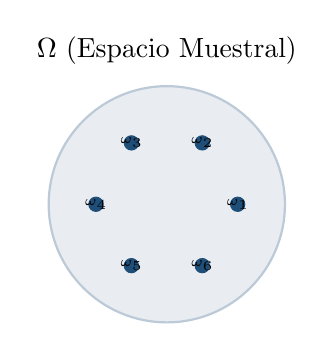
\begin{tikzpicture}[scale=0.75]
% Draw sample space
\draw[uddblue!30, fill=uddblue!10, thick] (0,0) circle (2);
\node[above] at (0, 2.2) {$\Omega$ (Espacio Muestral)};

% Draw sample points
\foreach \i in {1,2,3,4,5,6}{
  \pgfmathsetmacro{\angle}{360/6*(\i-1)}
  \pgfmathsetmacro{\x}{1.2*cos(\angle)}
  \pgfmathsetmacro{\y}{1.2*sin(\angle)}
  \filldraw[uddblue] (\x, \y) circle (0.12);
  \node[font=\tiny] at (\x, \y) {$\omega_\i$};
}
\end{tikzpicture}
\end{center}

\pause
\textbf{Ejemplo:} Lanzar un dado
$$\Omega = \{1, 2, 3, 4, 5, 6\}, \quad |\Omega| = 6$$
\end{column}
\end{columns}
\end{frame}

\begin{frame}[fragile]
\frametitle{Eventos y Operaciones}

\small
\begin{columns}[T]
\begin{column}{0.5\textwidth}
\begin{block}{Evento}
Subconjunto del espacio muestral: $A \subseteq \Omega$
\end{block}

\pause
\vspace{0.3cm}
\begin{itemize}
  \item Evento seguro: $A = \Omega$
  \item Evento imposible: $A = \emptyset$
  \item Evento elemental: $A = \{\omega\}$
\end{itemize}

\pause
\vspace{0.3cm}
\begin{block}{Operaciones entre Eventos}
\begin{itemize}
  \item Unión: $A \cup B$ (ocurre $A$ o $B$)
  \item Intersección: $A \cap B$ (ocurren $A$ y $B$)
  \item Complemento: $A^c$ (no ocurre $A$)
\end{itemize}
\end{block}
\end{column}

\begin{column}{0.5\textwidth}
\begin{center}
\textbf{Diagrama de Venn}
\pause

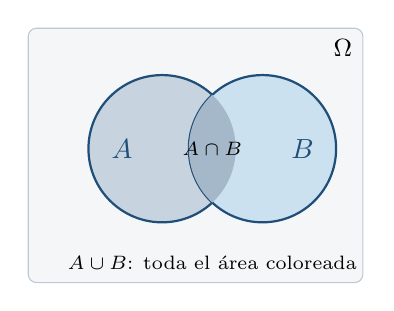
\begin{tikzpicture}[scale=0.85]
% Universe
\draw[uddblue!30, fill=uddblue!5, rounded corners=3pt] (-0.5,-0.8) rectangle (4.5,3);
\node[font=\small] at (4.2, 2.7) {$\Omega$};

% Circle A - larger with fill
\fill[uddblue!25] (1.5,1.2) circle (1.1);
\draw[uddblue, thick] (1.5,1.2) circle (1.1);

% Circle B - larger with fill
\fill[uddlight!25] (3,1.2) circle (1.1);
\draw[uddblue, thick] (3,1.2) circle (1.1);

% Intersection highlight
\begin{scope}
\clip (1.5,1.2) circle (1.1);
\fill[uddblue!40] (3,1.2) circle (1.1);
\end{scope}

% Labels
\node[font=\normalsize, text=uddblue] at (0.9, 1.2) {$A$};
\node[font=\normalsize, text=uddblue] at (3.6, 1.2) {$B$};
\node[font=\scriptsize] at (2.25, 1.2) {$A \cap B$};
\node[font=\scriptsize] at (2.25, -0.5) {$A \cup B$: toda el área coloreada};
\end{tikzpicture}

\pause
\vspace{0.3cm}
Propiedades (Leyes de De Morgan):
\begin{align*}
(A \cup B)^c &= A^c \cap B^c \\
(A \cap B)^c &= A^c \cup B^c
\end{align*}
\end{center}
\end{column}
\end{columns}
\end{frame}

\begin{frame}[fragile]
\frametitle{Axiomas de Kolmogorov}

\small
Sea $P: \mathcal{F} \to [0,1]$ una medida de probabilidad sobre $\Omega$.

\pause
\vspace{-0.1cm}
\begin{block}{Axioma 1: No-negatividad}
Para todo evento $A \in \mathcal{F}$: $P(A) \geq 0$
\end{block}

\pause
\vspace{-0.1cm}
\begin{block}{Axioma 2: Probabilidad del espacio total}
$P(\Omega) = 1$
\end{block}

\pause
\vspace{-0.1cm}
\begin{block}{Axioma 3: Aditividad ($\sigma$-aditividad)}
Para eventos disjuntos $A_i \cap A_j = \emptyset$ ($i \neq j$):
$$P\left(\bigcup_{i=1}^{\infty} A_i\right) = \sum_{i=1}^{\infty} P(A_i)$$
\end{block}

\pause
\vspace{-0.1cm}
\begin{block}{Consecuencias}
$P(\emptyset) = 0$, \quad $P(A) \leq 1$, \quad $P(A_1 \cup \cdots \cup A_n) = \sum_i P(A_i)$ (finitos disjuntos)
\end{block}
\end{frame}

\begin{frame}[fragile]
\frametitle{Regla de la Suma y del Complemento}

\small

\begin{block}{Regla de la Suma (Inclusión-Exclusión)}
Para dos eventos cualesquiera $A$ y $B$:
\pause
$$P(A \cup B) = P(A) + P(B) - P(A \cap B)$$
\end{block}

\pause
\begin{exampleblock}{Demostración intuitiva}
\begin{center}
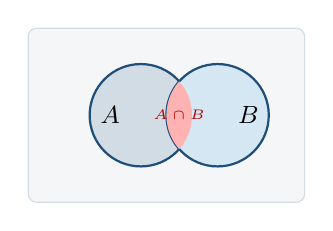
\begin{tikzpicture}[scale=0.65]
\draw[uddblue!20, fill=uddblue!5, rounded corners=3pt] (-1.2,-1.2) rectangle (4.2,2.2);
\fill[uddblue!20] (1,0.5) circle (1);
\draw[uddblue, thick] (1,0.5) circle (1);
\fill[uddlight!20] (2.5,0.5) circle (1);
\draw[uddblue, thick] (2.5,0.5) circle (1);
\begin{scope}
\clip (1,0.5) circle (1);
\fill[red!30] (2.5,0.5) circle (1);
\end{scope}
\node[font=\small] at (0.4, 0.5) {$A$};
\node[font=\small] at (3.1, 0.5) {$B$};
\node[font=\tiny, red!70!black] at (1.75, 0.5) {$A \cap B$};
\end{tikzpicture}

\scriptsize Si contamos $P(A)+P(B)$, la intersección se suma dos veces, por eso restamos $P(A \cap B)$.
\end{center}
\end{exampleblock}

\pause
\vspace{-0.1cm}
\begin{block}{Regla del Complemento}
$P(A^c) = 1 - P(A)$ \quad \textbf{Ejemplo:} Si 35\% apoyan una política, $P(\text{no apoyan}) = 0.65$
\end{block}
\end{frame}

% ==============================================================================
% SECTION 2: PROBABILIDAD CONDICIONAL
% ==============================================================================
\section{Probabilidad Condicional e Independencia}

\begin{frame}[fragile]
\frametitle{Probabilidad Condicional}

\begin{block}{Definición}
La probabilidad condicional de evento $A$ dado que ocurrió $B$ es:
$$P(A|B) = \frac{P(A \cap B)}{P(B)}, \quad P(B) > 0$$
\end{block}

\pause
\vspace{0.3cm}
\textbf{Interpretación:} Al saber que $B$ ocurrió, el espacio muestral se reduce a $B$. Preguntamos: ¿cuál es la probabilidad de que $A$ ocurra dentro de ese espacio reducido?

\pause
\begin{columns}[T]
\begin{column}{0.5\textwidth}
\begin{exampleblock}{Ejemplo: Género y Educación}
En una universidad:
\begin{itemize}
  \item 40\% estudia Ingeniería
  \item 25\% de Ingeniería son mujeres
  \item $P(\text{Mujer}|\text{Ingeniería})$ = 0.25
\end{itemize}

Pregunta: Si encuentro a una estudiante de Ingeniería al azar, ¿cuál es la probabilidad de que sea mujer?
\pause Respuesta: 0.25 (dentro de Ingeniería)
\end{exampleblock}
\end{column}

\begin{column}{0.5\textwidth}
\begin{center}
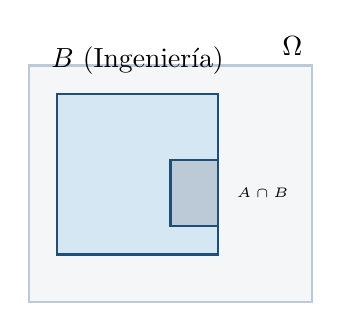
\begin{tikzpicture}[scale=1.2]
\draw[uddblue!30, fill=uddblue!5, thick] (0,0) rectangle (3,2.5);
\node[above left] at (3, 2.5) {$\Omega$};

\draw[uddblue, fill=uddlight!20, thick] (0.3,0.5) rectangle (2,2.2);
\node[above] at (1.15, 2.3) {$B$ (Ingeniería)};

\draw[uddblue, fill=uddblue!30, thick] (1.5,0.8) rectangle (2,1.5);
\node[right, font=\tiny] at (2.1, 1.15) {$A \cap B$};

\end{tikzpicture}

\vspace{0.3cm}
\small
$$P(A|B) = \frac{\text{Área } A \cap B}{\text{Área } B}$$
\end{center}
\end{column}
\end{columns}
\end{frame}

\begin{frame}[fragile]
\frametitle{Independencia de Eventos}

\small

\begin{block}{Definición}
Dos eventos $A$ y $B$ son \textbf{independientes} si:
$$P(A \cap B) = P(A) \cdot P(B)$$
O equivalentemente: $P(A|B) = P(A)$ y $P(B|A) = P(B)$
\end{block}

\pause
\vspace{-0.05cm}
\textbf{Interpretación:} Saber que $B$ ocurrió no cambia la probabilidad de que $A$ ocurra.

\pause
\vspace{-0.05cm}
\begin{exampleblock}{Ejemplo: Independencia}
Lanzar una moneda dos veces: $A$ = ``Primera cara'', $B$ = ``Segunda cara''.

$P(A) = 0.5$, $P(B) = 0.5$, $P(A \cap B) = 0.25 = P(A) \cdot P(B)$ $\checkmark$

Son independientes: el primer resultado no afecta el segundo.
\end{exampleblock}

\pause
\vspace{-0.05cm}
\begin{alertblock}{Atención: Correlación Espuria}
En ciencias sociales, es fácil confundir correlación con causalidad.
\textbf{Ejemplo:} Celulares y casos de cáncer aumentan juntos, pero dependen de una tercera variable (tiempo).
\end{alertblock}
\end{frame}

\begin{frame}[fragile]
\frametitle{Regla del Producto}

\small

\begin{block}{Regla del Producto}
$$P(A \cap B) = P(A|B) \cdot P(B) = P(B|A) \cdot P(A)$$

Para múltiples eventos:
$$P(A_1 \cap \cdots \cap A_n) = P(A_1) \cdot P(A_2|A_1) \cdot P(A_3|A_1 \cap A_2) \cdots$$
\end{block}

\pause
\begin{exampleblock}{Ejemplo: Muestreo sin reemplazo}
Extraer 2 cartas de una baraja (52 cartas):
\begin{itemize}
  \item $P(\text{As en 1ª}) = \frac{4}{52}$
  \pause
  \item $P(\text{As en 2ª} | \text{As en 1ª}) = \frac{3}{51}$
  \pause
  \item $P(\text{Dos ases}) = \frac{4}{52} \times \frac{3}{51} \approx 0.0045$
\end{itemize}
\end{exampleblock}

\pause
\smallskip
\textbf{Caso especial (independientes):} $P(A \cap B) = P(A) \cdot P(B)$
\end{frame}

% ==============================================================================
% SECTION 3: TEOREMA DE BAYES
% ==============================================================================
\section{Teorema de Bayes}

\begin{frame}[fragile]
\frametitle{Derivación del Teorema de Bayes}

\small

\begin{columns}[T]
\begin{column}{0.6\textwidth}
Comenzamos con la regla del producto:

\pause
$$P(A \cap B) = P(A|B) \cdot P(B)$$
$$P(A \cap B) = P(B|A) \cdot P(A)$$

\pause
Igualando ambas:
$$P(A|B) \cdot P(B) = P(B|A) \cdot P(A)$$

\pause
Despejando:
$$\boxed{P(B|A) = \frac{P(A|B) \cdot P(B)}{P(A)}}$$

\pause
\vspace{0.1cm}
\scriptsize
\textbf{Nomenclatura:}
$P(B)$=a priori, $P(A|B)$=verosimilitud, $P(A)$=evidencia, $P(B|A)$=a posteriori
\end{column}

\begin{column}{0.4\textwidth}
\begin{center}
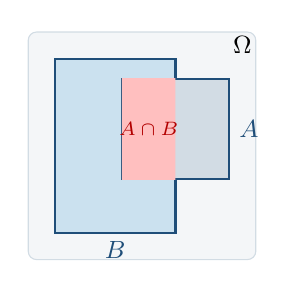
\begin{tikzpicture}[scale=0.85]
\draw[uddblue!20, fill=uddblue!5, rounded corners=3pt] (-0.2,-0.2) rectangle (3.2,3.2);
\node[font=\small] at (3, 3) {$\Omega$};

% Event B
\fill[uddlight!25] (0.2,0.2) rectangle (2,2.8);
\draw[uddblue, thick] (0.2,0.2) rectangle (2,2.8);
\node[font=\small, text=uddblue] at (1.1, -0.05) {$B$};

% Event A
\fill[uddblue!20] (1.2,1) rectangle (2.8,2.5);
\draw[uddblue, thick] (1.2,1) rectangle (2.8,2.5);
\node[font=\small, text=uddblue] at (3.1, 1.75) {$A$};

% Intersection highlight
\begin{scope}
\clip (0.2,0.2) rectangle (2,2.8);
\clip (1.2,1) rectangle (2.8,2.5);
\fill[red!25] (-1,-1) rectangle (4,4);
\end{scope}

\node[font=\scriptsize, red!70!black] at (1.6, 1.75) {$A \cap B$};
\end{tikzpicture}
\end{center}
\end{column}
\end{columns}
\end{frame}

\begin{frame}[fragile]
\frametitle{Teorema de Bayes Generalizado}

\small

\begin{block}{Ley de Probabilidad Total}
Si $B_1, B_2, \ldots, B_k$ particiona el espacio muestral:
$$P(A) = \sum_{i=1}^{k} P(A|B_i) \cdot P(B_i)$$
\end{block}

\pause
\vspace{-0.1cm}
\begin{block}{Teorema de Bayes (forma general)}
$$P(B_j|A) = \frac{P(A|B_j) \cdot P(B_j)}{\sum_{i=1}^{k} P(A|B_i) \cdot P(B_i)}$$
\end{block}

\pause
\vspace{0.05cm}
\textbf{Idea fundamental:} Actualizar creencias previas a luz de nueva evidencia.

\pause
\vspace{-0.05cm}
\begin{exampleblock}{Aplicación en ciencias sociales}
\textbf{A priori:} creencias antes de datos $\to$ \textbf{Datos:} nueva información $\to$ \textbf{A posteriori:} creencias actualizadas. Fundamento del análisis Bayesiano.
\end{exampleblock}
\end{frame}

\begin{frame}[fragile]
\frametitle{Ejemplo Aplicado: Prueba Diagnóstica}

\small

\textbf{Escenario:} Un test médico para detectar una enfermedad.

\pause
\textbf{Información dada:}
\begin{itemize}\setlength{\itemsep}{0pt}
  \item Prevalencia: $P(\text{Enfermo}) = 0.01$ (1\%)
  \item Sensibilidad: $P(\text{Positivo}|\text{Enfermo}) = 0.95$
  \item Especificidad: $P(\text{Negativo}|\text{Sano}) = 0.90$
\end{itemize}

\pause
\textbf{Pregunta:} Si da positivo, ¿probabilidad de estar realmente enfermo?

\pause
\textbf{Solución:} Probabilidad total:
$P(\text{Pos}) = 0.95 \times 0.01 + 0.10 \times 0.99 = 0.1085$

\pause
Aplicamos Bayes:
$P(\text{Enf}|\text{Pos}) = \frac{0.95 \times 0.01}{0.1085} \approx 0.0876$

\vspace{0.1cm}
\textbf{Resultado:} Solo 8.76\% de probabilidad, a pesar de test con 95\% sensibilidad.
\end{frame}

% ==============================================================================
% SECTION 4: VARIABLES ALEATORIAS
% ==============================================================================
\section{Variables Aleatorias}

\begin{frame}[fragile]
\frametitle{Concepto de Variable Aleatoria}

\begin{block}{Definición}
Una \textbf{variable aleatoria} es una función que asigna un número real a cada resultado en el espacio muestral:
$$X: \Omega \to \mathbb{R}$$
\end{block}

\pause
\vspace{0.3cm}
\begin{exampleblock}{Ejemplos}
\begin{itemize}
  \item Lanzar un dado: $X = $ resultado = 1, 2, 3, 4, 5, 6
  \item Encuesta: $X = $ número de personas que apoyan una medida
  \item Ingresos familiares: $X = $ ingreso mensual en pesos
  \item Temperatura diaria: $X = $ temperatura máxima en $^\circ$C
\end{itemize}
\end{exampleblock}

\pause
\vspace{0.3cm}
\begin{columns}[T]
\begin{column}{0.5\textwidth}
\begin{block}{Variable Aleatoria Discreta}
Toma valores en un conjunto numerable:
$$X \in \{x_1, x_2, x_3, \ldots\}$$
\end{block}
\end{column}

\begin{column}{0.5\textwidth}
\begin{block}{Variable Aleatoria Continua}
Toma valores en un intervalo de $\mathbb{R}$:
$$X \in [a, b] \text{ o } X \in \mathbb{R}$$
\end{block}
\end{column}
\end{columns}
\end{frame}

\begin{frame}[fragile]
\frametitle{Distribuciones de Probabilidad: Caso Discreto}

\small

\begin{block}{Función de Masa de Probabilidad (PMF)}
Para variable aleatoria discreta $X$:
$$P(X = x_i) = p_i, \quad \sum_{i} p_i = 1$$
\end{block}

\pause
\vspace{0.2cm}
\begin{exampleblock}{Ejemplo: Lanzar dos dados}
Sea $X = $ suma de los dos dados. Valores: 2, 3, ..., 12

\begin{center}
\tiny
\begin{tabular}{c|cccccccccccc}
$x$ & 2 & 3 & 4 & 5 & 6 & 7 & 8 & 9 & 10 & 11 & 12 \\
\hline
$P(X=x)$ & 1/36 & 2/36 & 3/36 & 4/36 & 5/36 & 6/36 & 5/36 & 4/36 & 3/36 & 2/36 & 1/36 \\
\end{tabular}
\end{center}
\end{exampleblock}

\pause
\vspace{-0.1cm}
\begin{block}{Función de Distribución Acumulada (CDF)}
$F(x) = P(X \leq x) = \sum_{x_i \leq x} P(X = x_i)$

$F$ es no-decreciente, $\lim_{x \to -\infty} F(x) = 0$, $\lim_{x \to \infty} F(x) = 1$
\end{block}
\end{frame}

\begin{frame}[fragile]
\frametitle{Distribuciones de Probabilidad: Caso Continuo}

\small

\begin{block}{Función de Densidad de Probabilidad (PDF)}
Para variable aleatoria continua $X$:
$$f(x) \geq 0, \quad \int_{-\infty}^{\infty} f(x) \, dx = 1$$
Probabilidad en un intervalo: $P(a \leq X \leq b) = \int_a^b f(x) \, dx$
\end{block}

\pause
\vspace{-0.05cm}
\textbf{Nota:} Para variable continua, $P(X = x) = 0$.

\pause
\vspace{-0.05cm}
\begin{block}{Función de Distribución Acumulada (CDF)}
$$F(x) = \int_{-\infty}^{x} f(t) \, dt, \quad \frac{dF}{dx} = f(x)$$
\end{block}

\pause
\vspace{-0.05cm}
\begin{exampleblock}{Ejemplo: Distribución Normal}
$f(x) = \frac{1}{\sigma\sqrt{2\pi}} \exp\!\left(-\frac{(x-\mu)^2}{2\sigma^2}\right)$, \quad parámetros: $\mu$ (media), $\sigma$ (desviación).
\end{exampleblock}
\end{frame}

\begin{frame}[fragile]
\frametitle{Valor Esperado (Esperanza)}

\small

\begin{block}{Definición: Caso Discreto}
$E(X) = \mu = \sum_{i} x_i \cdot P(X = x_i)$
\end{block}

\pause
\vspace{-0.1cm}
\begin{block}{Definición: Caso Continuo}
$E(X) = \mu = \int_{-\infty}^{\infty} x \cdot f(x) \, dx$
\end{block}

\pause
\vspace{-0.05cm}
\textbf{Interpretación:} Valor promedio. Centro de gravedad de la distribución.

\pause
\vspace{-0.05cm}
\begin{block}{Propiedades}
\begin{itemize}\setlength{\itemsep}{0pt}
  \item $E(c) = c$ (constante), \quad $E(aX + b) = aE(X) + b$ (linealidad)
  \item $E(X + Y) = E(X) + E(Y)$ (aditividad)
  \item Si $X$, $Y$ independientes: $E(XY) = E(X) E(Y)$
\end{itemize}
\end{block}

\pause
\vspace{-0.05cm}
\textbf{Ejemplo (dado):} $E(X) = \frac{1+2+\cdots+6}{6} = 3.5$
\end{frame}

\begin{frame}[fragile]
\frametitle{Varianza y Desviación Estándar}

\small

\begin{block}{Varianza}
Dispersión alrededor de la media:
$$\text{Var}(X) = \sigma^2 = E[(X - \mu)^2] = E(X^2) - [E(X)]^2$$
\end{block}

\pause
\vspace{-0.05cm}
\textbf{Unidades:} Cuadradas (si $X$ en pesos, Var($X$) en pesos$^2$)

\pause
\vspace{-0.05cm}
\begin{block}{Desviación Estándar}
$\sigma = \sqrt{\text{Var}(X)}$ — mismo tipo de unidades que $X$.
\end{block}

\pause
\vspace{-0.05cm}
\begin{block}{Propiedades}
\begin{itemize}\setlength{\itemsep}{0pt}
  \item $\text{Var}(c) = 0$
  \item $\text{Var}(aX + b) = a^2 \text{Var}(X)$
  \item Si independientes: $\text{Var}(X + Y) = \text{Var}(X) + \text{Var}(Y)$
\end{itemize}
\end{block}

\pause
\vspace{-0.05cm}
\textbf{Ejemplo (dado):} $E(X) = 3.5$, $E(X^2) \approx 15.17$, $\text{Var}(X) \approx 2.92$, $\sigma \approx 1.71$
\end{frame}

% ==============================================================================
% SECTION 5: CÓDIGO R
% ==============================================================================
\section{Implementación en R}

\begin{frame}[fragile]
\frametitle{Funciones R: Muestreo y Simulación}

\begin{block}{Muestreo aleatorio con \texttt{sample()}}
\begin{lstlisting}
# Simular 10 lanzamientos de moneda
moneda <- sample(c("Cara", "Cruz"), size=10, replace=TRUE)
print(moneda)

# Simular 100 lanzamientos de dado
dados <- sample(1:6, size=100, replace=TRUE)
prop.table(table(dados))  # Frecuencias relativas
\end{lstlisting}
\end{block}

\pause
\begin{block}{Repetición de experimentos con \texttt{replicate()}}
\begin{lstlisting}
# Simular la media de 100 lanzamientos de dado,
# repetido 1000 veces
medias <- replicate(1000, mean(sample(1:6, size=100,
                                       replace=TRUE)))
hist(medias, main="Distribución de medias muestrales")
\end{lstlisting}
\end{block}

\pause
\vspace{0.2cm}
\textbf{Salida esperada:} Histograma centrado en 3.5 (la media teórica del dado).
\end{frame}

\begin{frame}[fragile]
\frametitle{Simulación del Teorema de Bayes en R (Parte 1)}

\begin{lstlisting}[basicstyle=\ttfamily\tiny]
# Simulación: Prueba diagnóstica
set.seed(123)
n_simulaciones <- 100000

# Generar estado real de enfermedad (1% prevalencia)
enfermo <- rbinom(n_simulaciones, 1, p=0.01)

# Simular resultado de test
resultado_test <- numeric(n_simulaciones)

for(i in 1:n_simulaciones){
  if(enfermo[i] == 1){
    # Si enfermo: 95% positivo
    resultado_test[i] <- rbinom(1, 1, p=0.95)
  } else {
    # Si sano: 10% falso positivo
    resultado_test[i] <- rbinom(1, 1, p=0.10)
  }
}
\end{lstlisting}

\pause
\begin{exampleblock}{Lógica}
  Generamos 100.000 personas: 1\% enfermas (1000), 99\% sanas (99.000).
\end{exampleblock}
\end{frame}

\begin{frame}[fragile]
\frametitle{Simulación del Teorema de Bayes en R (Parte 2)}

\begin{lstlisting}
# Continuar desde frame anterior...

# Calcular P(Enfermo | Positivo)
prob_enfermo_dado_positivo <-
  sum(enfermo & resultado_test) /
  sum(resultado_test)

cat("P(Enfermo|Positivo) =",
    prob_enfermo_dado_positivo, "\n")
cat("Valor teórico = 0.0876\n")
\end{lstlisting}

\pause
\begin{exampleblock}{Interpretación}
  El resultado simulado debe coincidir con el teórico (\(\approx 8.76\%\)).

  Esto valida el Teorema de Bayes.
\end{exampleblock}
\end{frame}

\begin{frame}[fragile]
\frametitle{Distribuciones en R}

\small

\begin{block}{Funciones de distribución}
En R, las distribuciones tienen prefijos estándar:
\begin{itemize}
  \item \texttt{d*} — función de densidad/masa
  \item \texttt{p*} — función acumulada (CDF)
  \item \texttt{q*} — función cuantil
  \item \texttt{r*} — números aleatorios
\end{itemize}
\end{block}

\pause
\begin{lstlisting}[basicstyle=\ttfamily\tiny]
# Distribución normal: X ~ N(100, 15^2)
media <- 100; desv_est <- 15
dnorm(100, mean=100, sd=15)
pnorm(115, mean=100, sd=15)
qnorm(0.95, mean=100, sd=15)
muestra <- rnorm(1000, mean=100, sd=15)
hist(muestra, freq=FALSE)
curve(dnorm(x, mean=100, sd=15),
      add=TRUE, col="blue")
\end{lstlisting}
\end{frame}

% ==============================================================================
% SECTION 6: EJERCICIO PRÁCTICO
% ==============================================================================
\section{Ejercicio Práctico}

\begin{frame}[fragile]
\frametitle{Ejercicio Práctico: Análisis de Encuesta}

\small

\textbf{Escenario:} Encuesta a 500 ciudadanos sobre intención de voto.

\pause
\vspace{0.1cm}
\textbf{Datos:}
\begin{itemize}
  \item 210 con intención de voto
  \item De estos, 140 tienen educación superior
  \item Sin intención: 180 con educación superior
  \item Total educación superior: 320
\end{itemize}

\pause
\vspace{0.15cm}
\textbf{Preguntas:}
\begin{enumerate}
  \item Calcule $P(V)$ y $P(E)$
  \item ¿Son independientes?
  \item Calcule $P(V|E)$ y $P(E|V)$
  \item ¿Relación entre educación e intención de voto?
\end{enumerate}

\pause
\vspace{0.1cm}
\textbf{Para resolver:} Tabla de contingencia, operaciones de probabilidad, verificar independencia.
\end{frame}

\begin{frame}[fragile]
\frametitle{Solución del Ejercicio (Parte 1)}

\small

\begin{block}{Tabla de Contingencia}
\centering
\tiny
\begin{tabular}{c|cc|c}
& Educación Sup. & Sin Educación Sup. & Total \\
\hline
Vota & 140 & 70 & 210 \\
No vota & 180 & 110 & 290 \\
\hline
Total & 320 & 180 & 500 \\
\end{tabular}
\end{block}

\pause
\vspace{0.2cm}
\begin{block}{Probabilidades Marginales}
$P(V) = 0.42$, $P(E) = 0.64$, $P(V^c) = 0.58$, $P(E^c) = 0.36$
\end{block}

\pause
\begin{block}{Verificar Independencia}
$$P(V \cap E) = 0.28 \quad \text{vs} \quad P(V) \cdot P(E) = 0.2688$$

No independientes (aunque cercanos).
\end{block}
\end{frame}

\begin{frame}[fragile]
\frametitle{Solución del Ejercicio (Parte 2)}

\small

\begin{block}{Probabilidades Condicionales}
$$P(V|E) = \frac{140}{320} = 0.4375 \quad P(E|V) = \frac{140}{210} = 0.6667$$
\end{block}

\pause
\vspace{0.15cm}
\begin{block}{Interpretación}
\begin{itemize}
  \item Con educación superior, 43.75\% vota
  \item Votantes, 66.67\% con educación superior
  \item Vs $P(V) = 42\%$ → aumenta ligeramente
\end{itemize}
\end{block}

\pause
\begin{alertblock}{Conclusión}
Asociación débil pero positiva. Preguntas: ¿Causal? ¿Confundidoras? ¿Regional? ¿Temporal?
\end{alertblock}
\end{frame}

% ==============================================================================
% SUMMARY SLIDE
% ==============================================================================
\begin{frame}[fragile]
\frametitle{Resumen de Conceptos Clave}

\small

\begin{columns}[T]
\begin{column}{0.5\textwidth}
\begin{block}{Fundamentos}
\begin{itemize}
  \item Espacio muestral, eventos
  \item Axiomas de Kolmogorov
  \item Regla suma y complemento
\end{itemize}
\end{block}

\begin{block}{Condicionalidad}
\begin{itemize}
  \item $P(A|B) = P(A \cap B) / P(B)$
  \item Independencia: $P(A \cap B) = P(A) \cdot P(B)$
  \item Regla del producto
\end{itemize}
\end{block}
\end{column}

\begin{column}{0.5\textwidth}
\begin{block}{Bayes y V.A.}
\begin{itemize}
  \item Teorema de Bayes
  \item V.A. discretas y continuas
  \item PMF, PDF, CDF
\end{itemize}
\end{block}

\begin{block}{Características}
\begin{itemize}
  \item $E(X)$ — valor esperado
  \item $\text{Var}(X)$ — varianza
  \item $\sigma$ — desviación estándar
\end{itemize}
\end{block}
\end{column}
\end{columns}

\pause
\vspace{0.2cm}
\centering
\normalsize \textbf{Próxima sesión:} Distribuciones comunes (Normal, Binomial, Poisson)
\end{frame}

\end{document}
